\chapter{Tensiones y sobretensiones}
    En este tema se presentan las tensiones nominales y tensiones más elevadas de las redes eléctricas de alta tensión, las tensiones más elevadas del material a instalar en ellas, las tensiones nominales del aislamiento y las distancias mínimas de aislamiento en aire que la normativa aplicable establece.

    \section{Clasificación del material de alta tensión.}
        Las tensiones más elevadas de los materiales a instalar en las redes trifásicas de alta tensión dependen de las tensiones más elevadas de las redes y de las sobretensiones esperadas en ellas.

        \subsection{Tensión nominal de una red o instalación.}
            Representada por $U_\textit{n}$, la tensión nominal de una red es el valor convencional de la tensión con la que se denomina un sistema o instalación y para el que ha sido previsto su funcionamiento y aislamiento.\newline

            La tensión nominal de la red está establecida en los reglamentos españoles de Baja Tensión (BT) y Alta Tensión (AT). Para la red trifásica de BT se establece en $400\,\textit{V}$, mientras que para el reglamento de AT se establecen una amplia gama de niveles, normalmente de $10$, $15$, $20$, $25$ y $30\,\textit{kV}$ para las redes de distribución de media tensión (MT); $45$, $66$, $132$ y $150\,\textit{kV}$ para las redes de distribución de alta tensión (AT) y de $220$ y $400\,\textit{kV}$ para las redes de transporte, aunque existen excepciones, ya que las redes de $220\,\textit{kV}$ también se usan para redes de distribución de AT y en las Islas Canarias y Baleares se utilizan tensiones de transporte con niveles por debajo de $220\,\textit{kV}$. Normas internacionales establecen además otros niveles de tensiones nominales a las consideradas en los reglamentos españoles, que no son aplicadas en España.

        \subsection{Tensión más elevada de una red trifásica.}
            Representada por $U_\textit{s}$, la tensión más elevada de una red trifásica es el valor eficaz más elevado de la tensión entre fases que puede presentarse en un instante y en un punto cualquiera de la red, en las condiciones normales de explotación. Este valor no tiene en cuenta las variaciones transitorias (por ejemplo, las tensiones transitorias que aparecen durante las maniobras en la red), ni las variaciones temporales de tensión debidas a condiciones anormales de la red (averías o desconexiones bruscas de cargas importantes, sobretensiones por faltas asimétricas, etc.).\newline
            
            Existe una relación directa entre la tensión nominal de la red, $U_\textit{n}$, y la tensión más elevada de la red $U_\textit{s}$. Dicha relación para instalaciones de alta tensión viene recogida en la Tabla \ref{tab:tensionMasElevada}, de manera que a cada tensión nominal normalizada de la red le corresponde un valor de tensión más elevado de la red.

            \begin{table}[H]
                \centering
                \renewcommand{\arraystretch}{1.1}
                \begin{tabular}{ccc}
                    Distribución y transporte & $U_\textit{n}\,[\textit{kV}]$ & $U_\textit{s}\,[\textit{kV}]$\\
                    \hline
                    \multirow{5}{*}{Distribución de MT} & 10 & 12\\
                    & 15 & 17.5 \\
                    & 20 & 24 \\
                    & 25 & 30 \\
                    & 30 & 36 \\
                    \hline
                    \multirow{5}{*}{Distribución de AT} & 45 & 52 \\
                    & 66 & 72.5 \\
                    & 110 & 123 \\
                    & 132 & 145 \\
                    & 150 & 170 \\
                    \hline
                    \multirow{2}{*}{Transporte de AT}& 220 & 245 \\
                    & 400 & 420 \\ 
                \end{tabular}
                \caption{Tensiones más elevadas de la red.}
                \label{tab:tensionMasElevada}
            \end{table}

        \subsection{Tensión más elevada del material.}
            Representada por $U_\textit{m}$, la tensión más elevada del material corresponde con la mayor tensión eficaz entre fases para el cual se define el material, en lo que se refiere al aislamiento y determinadas características que están eventualmente relacionadas con esta tensión, en las normas propuestas para cada material. Esta tensión puede estar aplicada al material de forma permanentemente sin que su aislamiento sufra daño apreciable.\newline
            
            Dependiendo del tipo de material se utiliza también como parámetro adicional el valor de la tensión asignada del material, también conocida por tensión nominal del material. Tal es el caso de los cables aislados de alta tensión, los transformadores de potencia, los transformadores de medida y los de protección y los fusibles (limitadores o de expulsión). Para la paramenta (seccionadores, interruptores, interruptores automáticos, etc.) el valor de la tensión más elevada del material corresponde con la tensión nominal o tensión asignada.\newline
            
            No se debe confundir la tensión más elevada de la red con la tensión más elevada del material. La tensión más elevada del material debe ser igual o superior a la tensión más elevada de la red, dependiendo de las sobretensiones esperadas en la red\footnote{Las redes eléctricas de media tensión de tensión nominal $U_\textit{n} = 15\,\textit{kV}\,(U_\textit{s} = 17.5\,\textit{kV})$ utilizan aparamenta de de tensión más elevada del material de $U_\textit{m} = 24\,\textit{kV}$.}.
            
            \begin{equation}
                U_\textit{m} \geq U_\textit{s}
            \end{equation}

        \subsection{Clasificación de los materiales por grupos.}
        Los materiales se clasifican en tres grupos en función del nivel de tensión más elevado del material: A, B y C. Para cada uno de estos grupos se establecen diferentes niveles de aislamiento nominal, como se ve en la Tabla \ref{tab:gruposTensiones}.\newline

        \begin{table}[H]
            \centering
            \renewcommand{\arraystretch}{1.1}
            \begin{tabular}{cc}
                Grupo & $U_\textit{m}\,[\textit{kV}]$\\
                \hline
                A & $1 \leq U_\textit{m} < 36$\\
                B & $36 \leq U_\textit{m} < 245$\\
                C & $U_\textit{m} > 245$\\
            \end{tabular}
            \caption{Grupos de materiales en función de su tensión más elevada del material.}
            \label{tab:gruposTensiones}
        \end{table}
        
        Según el RAT, salvo casos especiales debidamente justificados por el proyectista, se exige que las instalaciones estén diseñadas con niveles de tensiones de aislamiento nominales elegidos conformes a los criterios establecidos por las normas de coordinación de aislamiento UNE-EN 60071-1 y UNE-EN 60071-2. Estas normas tienen en cuenta las condiciones específicas de ubicación geográfica de la instalación (altitud, nivel de contaminación y nivel ceraúnico) y el emplazamiento dentro de la red que condiciona las sobretensiones que pueden aparecer\footnote{En el tema 7 de coordinación de aislamiento se desarrolla los conceptos para que el riesgo de fallo dieléctrico esté dentro de niveles aceptables.}.\newline
        
        Para cada uno de los tres grupos se establecen unos niveles de tensión de aislamiento diferentes junto con unos ensayos dieléctricos que deben ser capaces de soportar el material. Estos niveles de tensión de ensayo tienen en cuenta las sobretensiones que pueden aparecer en la red.

    \section{Sobretensiones en redes de alta tensión.}
        \subsection{Tipos de sobretensiones en redes eléctricas de alta tensión.}
            Las sobretensiones que pueden aparecer en las redes e instalaciones eléctricas de alta tensión se clasifican en sobretensiones temporales, sobretensiones transitorias de frente lento (por ejemplo las debidas a las maniobras de cierre y apertura de interruptores), sobretensiones transitorias de frente rápido (como las provocadas por el rayo) y sobretensiones transitorias de frente muy rápido (\textit{Very Fast Transients}, producidas, por ejemplo, por las maniobras de seccionadores realizadas en el interior de los conductos de las subestaciones aisladas en gas, GIS, a alta presión\footnote{El hexafluoruro de azufre ($\textit{SF}_6$) es un gas aislante tradicionalmente utilizado en las GIS, de excelentes propiedades dieléctricas y frente a la extinción del arco eléctrico de las maniobras de corte. Es estable, inoloro, incoloro, más pesado que el aire. Sin embargo, las fugas de $\textit{SF}_6$ al aire ambiente diluyéndose con éste contribuye con el efecto invernadero afectando al calentamiento global. Por esta razón, en la actualidad se utilizan en las nuevas GIS gases alternativos ecológicos.}).\newline

            Lo primero que cabe destacar en esta clasificación es la diferencia establecida entre las sobretensiones temporales y las sobretensiones transitorias. Para entender esta diferencia se debe tomar como referencia el intervalo de tiempo de un ciclo de tensión de red, que para redes de $50\,\textit{Hz}$, corresponde con un período de $20\,\textit{ms}$. Sobre este periodo de red se establece el carácter más o menos transitorio de las sobretensiones. Por ejemplo, las sobretensiones temporales permanecen durante varios ciclos de red, mientras que las sobretensiones de duración inferior a un periodo de red se califican como transitorias.\newline

            El caso más característico de las sobretensiones temporales en una red trifásica es la originada por un cortocircuito fase-tierra. Durante este se producirá una sobretensión en las fases sanas. La duración de la corriente de cortocircuito depende del tiempo que tardan las protecciones en despejarlo, el cual, si las protecciones siguen una característica de tiempo inverso, dependerá a su vez de la amplitud de la corriente de la falta.\newline
            
            Excepto en los casos de faltas a tierra de baja corriente de falta\footnote{Las faltas a tierra de bajo valor de corriente pueden ser debidas a fallos a través de impedancias de alto valor, como faltas a través de ramas de árbol o aislamientos defectuosos, o en redes con neutro aislado con baja capacidad entre las fases y tierra.}, la duración de la falta será, normalmente inferior a $3\,\textit{s}$. En media tensión normalmente las faltas se despejan en un intervalo de tiempo inferior a $1\,\textit{s}$ y en alta tensión la duración es inferior a $0.5\,\textit{s}$. Los órdenes de magnitud para despejar un cortocircuito normalmente se encontrarán entre $1\,\textit{s}$ y $0.1\,\textit{s}$, tiempos que para red de $50\,\textit{Hz}$ equivalen a $50$ y $5$ ciclos de red, respectivamente, por lo que la duración de la sobretensión en las fases sanas debida a un cortocircuito fase-tierra probablemente durará varios periodos de red, lo que justifica la denominación de sobretensión temporal.\newline

            Sin embargo, una sobretensión transitoria como, por ejemplo, la derivada de un rayo, tiene una duración muy inferior al periodo de la red. Los rayos son pulsos positivos o negativos, que presenta un tiempo de frente, $T_1$, breve, entre $0.1$ y $2\,\mu\textit{s}$, y un tiempo hasta el valor mitad de su cresta, $T_2$, algo más largo, del orden de decenas de microsegundos y nunca superior a $300\,\mu\textit{s}$\footnote{Los impulsos tipo rayo normalizados $T_1 = 1.2\,\mu\textit{s}$ y $T_2 = 50\,\mu\textit{s}$ siguen una forma de onda unidireccional de doble exponencial $u(t) = A_0 \cdot e^{-t/\alpha} \cdot e^{-t/\beta}$, con $\alpha = 68,48\,\mu\textit{s}$ y $\beta = 0.40\,\mu\textit{s}$}, de forma que en unos $500\,\mu\textit{s}$ desde el inicio del rayo la sobretensión del rayo habrá desaparecido. Si se compara la duración total del pulso de un rayo ($<0.5\,\textit{ms}$) con el periodo de red ($20\,\textit{ms}$) es fácil comprender el carácter transitorio del rayo, según se muestra en la Fig. \ref{fig:sobretensiones}.

            \begin{figure}[H]
                \centering
                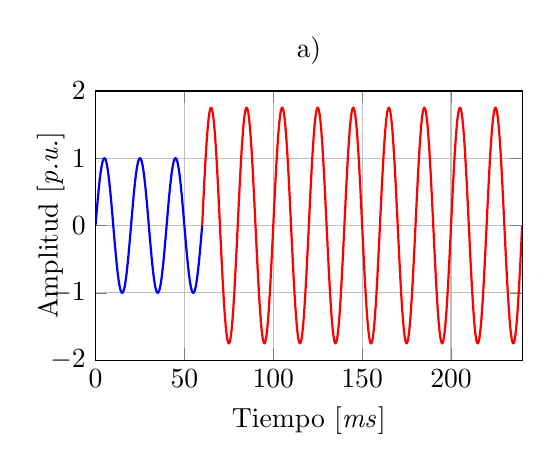
\begin{tikzpicture}
                    \begin{axis}[
                        width = 7cm,
                        height = 5cm,
                        xlabel={Tiempo [\textit{ms}]},
                        ylabel={Amplitud [\textit{p.u.}]},
                        ylabel style={yshift=-12pt},
                        grid=both,
                        xmin=0, xmax=240,
                        ymin=-2, ymax=2,
                        domain=0:240,
                        samples=1000,
                        title={a)},
                    ]
                    \addplot [blue, thick, domain = 0:60] 
                    {
                        (x < 60) * sin(deg(2 * pi * 50 * x / 1000))                        
                    };
                    \addplot [red, thick, domain = 60:240] 
                    {
                        (x >= 60) * sin(deg(2 * pi * 50 * x / 1000)) * (1 + 0.75)
                    };
                    \end{axis}
                \end{tikzpicture}
                \hspace{0.5cm}
                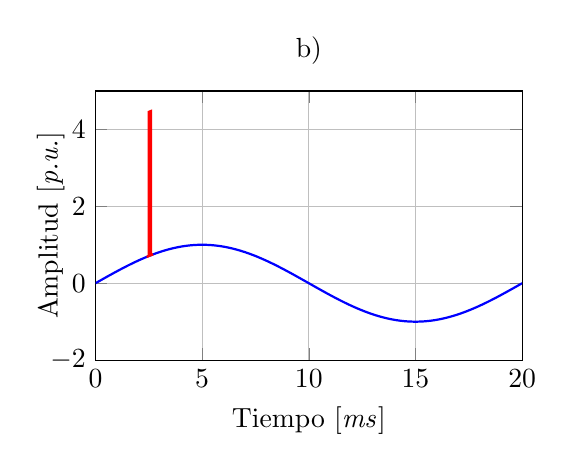
\begin{tikzpicture}
                    \begin{axis}[
                        width = 7cm,
                        height = 5cm,
                        xlabel={Tiempo [\textit{ms}]},
                        ylabel={Amplitud [\textit{p.u.}]},
                        ylabel style={yshift=-12pt},
                        grid=both,
                        xmin=0, xmax=20,
                        ymin=-2, ymax=5,
                        domain=0:240,
                        samples=1000,
                        title={b)},
                    ]
                    \addplot [blue, thick, domain = 0:20] 
                    {
                        sin(deg(2 * pi * 50 * x / 1000))                        
                    };
                    \addplot [red, thick, domain = 2.4:2.7] 
                    {
                        3.75 * (x >= 2.5) * (x <= 2.6) + sin(deg(2 * pi * 50 * x / 1000))
                    };
                    \end{axis}
                \end{tikzpicture}
                \caption{Sobretensiones. a) Temporal derivada de un cortocircuito fase-tierra. b) Transitoria de frente rápido provocada por un rayo.}
                \label{fig:sobretensiones}
            \end{figure}

            Las sobretensiones transitorias de frente lento están asociadas, normalmente, con las maniobras de la aparamenta, por ejemplo, las que aparecen en el extremo de una línea al cerrar o abrir un interruptor en el extremo opuesto. Su duración de unos pocos milisegundos permite clasificarlas también dentro del grupo de las sobretensiones transitorias, pero más lentas que las originadas por el rayo. Por el contrario, las sobretensiones transitorias de frente muy rápido son mucho más escarpadas que las provocadas por el rayo, con frentes de onda extremadamente breves de unos pocos nanosegundos.

        \subsection{Sobretensiones temporales. Faltas fase-tierra.}
            La sobretensión debida a un cortocircuito fase-tierra es la sobretensión temporal más representativa de este tipo\footnote{Dentro de las sobretensiones temporales también se incluyen las sobretensiones por ferroresonancias producidas por fenómenos de saturación de núcleos ferromagnéticos (ver Tema 5). Por lo general, las ondas sinusoidales que se producen en las ferroresonancias son múltiplos o submúltiplos de la frecuencia de red.}. La falta de una fase a tierra en un sistema trifásico produce una sobretensión en las fases sanas (fases sin defecto). Los conductores de estas fases adquirirán una tensión superior a la que tenían antes del fallo.\newline
            
            En general la tensión de cada fase en régimen normal de funcionamiento es, a lo sumo, $U_\textit{s}/\sqrt{3}$. En un sistema trifásico equilibrado, esté o no referenciado a tierra, siempre existen capacidades a tierra, como las propias de los cables aislados de las redes de alta tensión con sus pantallas puestas a tierra, que condicionan a que en condiciones normales la tensión sea $U_\textit{s}/\sqrt{3}$, aunque el neutro de la red de alimentación no estuviera referido a tierra.\newline

            Cuando se produce un cortocircuito fase-tierra, las fases sanas incrementan su tensión en función del tipo de conexión a tierra del neutro de la red. En la Fig. \ref{fig:cortoFTAislado} se representa una red trifásica con neutro aislado. Aunque muchas redes eléctricas utilizan el neutro puesto a tierra a través de una impedancia se utiliza este caso para por su simplicidad de análisis en caso de cortocircuito fase tierra.

            \begin{figure}
                \centering
                \begin{tikzpicture}[straight voltages]
                    \draw (0,0) to[sV, l={R}] ++(2,0) -- ++(3,0)coordinate(scPoint);
                    \draw (0,-1.5) to[sV, l={S}] ++(2,0) -- ++(2,0) to[european resistor, l_={$Z_\textit{pant}$}, v^={$\dfrac{U_\textit{s}}{\sqrt{3}}$}] ++(0,-2) node[tlground]{};
                    \draw (0,-3) to[sV, l={T}] ++(2,0)coordinate(endT);
                    \draw[dashed] (endT) -- ++(1,0);
                    \draw (0,0) -- (0,-3);
                    \node at (0,-1.5) [circ]{};
                    \node at (0,-1.5) [left]{N};
                    \draw ($(scPoint)+(0,-0.15)$) -- ++(-0.2,-0.4) -- ++(0.2,0.1)coordinate(beginArrow);
                    \draw[->, >=Stealth] (beginArrow) -- ++(-0.2,-0.4)coordinate(endArrow);
                    \node at ($(endArrow)+(0,-0.1)$) [tlground]{};   
                    \draw[->, >=Stealth] ($(scPoint)+(-2.5,-0.25)$) to[short, l={$U_\textit{s}$}] ++(0,-1);
                \end{tikzpicture}
                \caption{Cortocircuito fase-tierra con neutro aislado.}
                \label{fig:cortoFTAislado}
            \end{figure}

            Supóngase que se produce el fallo fase a tierra en la fase R mostrada en la Fig. \ref{fig:cortoFTAislado}. Desde el momento en que se produce el cortocircuito, la fase en defecto estará referida a tierra, al mismo potencial que los aislamientos de las fases sanas. Eso significa que desde el momento del cortocircuito y en los instantes siguientes, los aislamientos de las fases sanas tendrán que soportar la tensión entre fases de la red, que como ya se ha dicho podrá ser $U_\textit{s}$.\newline
            
            En consecuencia, después de la falta la tensión de las fases sanas es $U_\textit{s}$, mientas que antes de la falta era $U_\textit{s}/\sqrt{3}$. La tensión en las fases sanas se ha incrementado $\sqrt{3}$ veces respecto de la tensión que inicialmente tenía. Este factor de elevación la tensión recibe el nombre de coeficiente de defecto tierra ($k$), que es la relación entre la tensión máxima que aparece en las fases sanas tras la falta respecto de la tensión máxima que tenían antes de la falta.

            \begin{equation}
                k = \dfrac{U_\textit{máx, con falta}}{U_\textit{máx, sin falta}}
            \end{equation}

            Si el neutro no estuviera aislado, sino conectado a tierra a través de una impedancia, la tensión en las fases sanas no hubiera sido tan elevada. Para conocer la tensión en las fases sanas después de un cortocircuito debería aplicarse el método de las componentes simétricas, el cual no es temario de esta asignatura. En el anexo A de la norma IEC 60071-2 se establecen gráficas para conocer el coeficiente de defecto a tierra a partir de las relaciones entre las impedancias de secuencia directa, inversa y homopolar de puesta a tierra.\newline

            Cuando el neutro de la red está aislado, en caso de cortocircuito monofásico la sobretensión en las fases sanas es mayor que cuando está conectado rígidamente a tierra a través de una impedancia, pero la corriente de defecto es menor, por lo que las protecciones pueden tardar un mayor tiempo en despejar el cortocircuito. En redes con neutro aislado, en general, las sobretensiones son más elevadas y perduran por más tiempo (minutos, horas o incluso no ser despejadas).

        \subsection{Sobretensiones transitorias de frente lento. Maniobras en interruptores.} 
            Una conexión o reenganche de una línea trifásica produce sobretensiones de maniobra en las tres fases de la línea. Por lo tanto, cada maniobra produce tres sobretensiones fase- tierra y las tres sobretensiones correspondientes fase-fase. En la Fig. \ref{fig:sobretensionesManiobra} se muestran las tensiones de fase en una instalación durante los primeros periodos de su energización. Inicialmente se encuentra fuera de servicio ($U_\textit{R} = U_\textit{S} = U_\textit{T} = 0$) y al efectuar el cierre del interruptor situado en una subestación lejana, se producirán ondas sinusoidales deformadas en cada una de las fases, que evidencian procesos transitorios.\newline
            
            \pgfmathdeclarefunction{blend}{3}{%
            \pgfmathparse{(#1)*(1 - (#3)) + (#2)*(#3)}%
            }
            \begin{figure}[H]
                \centering
                \begin{tikzpicture}
                    \begin{axis}[
                        width = 5cm,
                        height = 4cm,
                        xlabel={Tiempo [\textit{ms}]},
                        ylabel={Amplitud [\textit{p.u.}]},
                        ylabel style={yshift=-12pt},
                        grid=both,
                        xmin=0, xmax=60,
                        ymin=-2, ymax=2,
                    domain=0:60,
                    samples=1000,
                    title={R},
                    ]
                    \addplot[thick, blue] { (x<=20) * (sin(deg(2*pi*50*x/1000)) + 1.5 * sin(deg(6*pi*50*x/1000)) * exp(-50*x/1000)) + (x>20 && x<=25) * blend((sin(deg(2*pi*50*x/1000)) + 1.5 * sin(deg(6*pi*50*x/1000)) * exp(-50*x/1000)), sin(deg(2*pi*50*x/1000)), (x-20)/5) + (x>25) * sin(deg(2*pi*50*x/1000))};
                \end{axis}
            \end{tikzpicture}
            \hspace{0.5cm}
            \begin{tikzpicture}
                \begin{axis}[
                    width = 5cm,
                    height = 4cm,
                    xlabel={Tiempo [\textit{ms}]},
                    ylabel={Amplitud [\textit{p.u.}]},
                    ylabel style={yshift=-12pt},
                    grid=both,
                    xmin=0, xmax=60,
                    ymin=-2, ymax=2,
                    domain=0:60,
                    samples=1000,
                    title={S},
                    ]
                    \addplot[thick, red] { (x<=20) * (sin(deg(2*pi*50*(x-4)/1000)) + 1.5 * sin(deg(6*pi*50*(x-4)/1000)) * exp(-50*x/1000)) + (x>20 && x<=25) * blend((sin(deg(2*pi*50*(x-4)/1000)) + 1.5 * sin(deg(6*pi*50*(x-4)/1000)) * exp(-50*x/1000)), sin(deg(2*pi*50*(x-4)/1000)), (x-20)/5) + (x>25) * sin(deg(2*pi*50*(x-4)/1000))};
                \end{axis}
            \end{tikzpicture}
            \hspace{0.5cm}
            \begin{tikzpicture}
                \begin{axis}[
                    width = 5cm,
                    height = 4cm,
                    xlabel={Tiempo [\textit{ms}]},
                    ylabel={Amplitud [\textit{p.u.}]},
                    ylabel style={yshift=-12pt},
                    grid=both,
                    xmin=0, xmax=60,
                    ymin=-2, ymax=2,
                    domain=0:60,
                    samples=1000,
                    title={T},
                    ]
                    \addplot[thick, green] { (x<=20) * (sin(deg(2*pi*50*(x+4)/1000)) + 1.5 * sin(deg(6*pi*50*(x+4)/1000)) * exp(-50*x/1000)) + (x>20 && x<=25) * blend((sin(deg(2*pi*50*(x+4)/1000)) + 1.5 * sin(deg(6*pi*50*(x+4)/1000)) * exp(-50*x/1000)), sin(deg(2*pi*50*(x+4)/1000)), (x-20)/5) + (x>25) * sin(deg(2*pi*50*(x+4)/1000))};
                \end{axis}
            \end{tikzpicture}
            \caption{Formas de onda de las sobretensiones transitorias de la energización de una instalación por la maniobra de un interruptor trifásico.}
            \label{fig:sobretensionesManiobra}
            \end{figure}

            Algunos elementos como las capacidades tendrán que cargarse, las reactancias o transformadores de potencia deberán magnetizarse\dots con sus constantes de tiempo correspondientes. Además, se producirá la propagación de una onda viajera de tensión debido a la conexión a través de cada una de las fases que, al llegar al extremo de la instalación, provocarán reflexión, completa si el interruptor de entrada de la subestación estuviera abierto, o parcial si estuviera cerrado pero la impedancia característica de la subestación es diferente a la de la línea\footnote{La impedancia característica de una línea aérea es del orden de $400\,\Omega$, mientras que la de una GIS es del orden de $50\,\Omega$, y la de un cable aislado del orden de $25\,\Omega$)}.\newline
            
            Estos transitorios son complejos de analizar por métodos analíticos, por lo que se recurre a software especializado, que utiliza modelos eléctricos para los diferentes componentes y elementos de la red (ver Fig. \ref{fig:modelosTransitorios}). Los pararrayos, si existen, deben también ser modelados, ya que estos elementos limitarán las sobretensiones transitorias de la red.
            
            \begin{figure}[H]
                \centering
                \begin{minipage}{0.7\textwidth}
                    \centering
                    a)
                    
                    \vspace{0.25cm}
                    \begin{tikzpicture}
                        \draw (0,0)node[tlground, rotate=-90]{} to[C, -*] ++(2,0)coordinate(beginC) to[C] ++(6,0)coordinate(beginC2) to[C, *-] ++(2,0)node[tlground, rotate=90]{};
                        \draw (0,-2)node[tlground, rotate=-90]{} to[C, -*] ++(2,0) to[C] ++(6,0) to[C, *-] ++(2,0)node[tlground, rotate=90]{};
                        \draw (0,-4)node[tlground, rotate=-90]{} to[C, -*] ++(2,0) to[C] ++(6,0) to[C, *-] ++(2,0)node[tlground, rotate=90]{};
                        \draw (0,-6)node[tlground, rotate=-90]{} to[C, -*] ++(2,0) to[C] ++(6,0) to[C, *-] ++(2,0)node[tlground, rotate=90]{};
                        \draw (0,-8)node[tlground, rotate=-90]{} to[C, -*] ++(2,0) to[C] ++(6,0) to[C, *-] ++(2,0)node[tlground, rotate=90]{};
                        
                        \draw (beginC) to[C] ++(0,-2) to[C] ++(0,-2)coordinate(beginD1);
                        \draw (beginD1) -- ++(0,-0.5)coordinate(int1D1);
                        \draw[dash pattern=on 3.5pt off 3.5pt] (int1D1) -- ++(0,-1)coordinate(int2D1);
                        \draw (int2D1) -- ++(0,-0.5)coordinate(endD1);
                        \draw (endD1) to[C] ++(0,-2) to[C] ++(0,-2)node[tlground]{};
                        
                        \draw (beginC2) to[C] ++(0,-2) to[C] ++(0,-2)coordinate(beginD2);
                        \draw (beginD2) -- ++(0,-0.5)coordinate(int1D2);
                        \draw[dash pattern=on 3.5pt off 3.5pt] (int1D2) -- ++(0,-1)coordinate(int2D2);
                        \draw (int2D2) -- ++(0,-0.5)coordinate(endD2);
                        \draw (endD2) to[C] ++(0,-2) to[C] ++(0,-2)node[tlground]{};
                        
                        \draw ($(beginC)+(1.5,0)$) to[L, -*] ++(0,-2) to[L, -*] ++(0,-2)coordinate(beginD3);
                        \draw (beginD3) -- ++(0,-0.5)coordinate(int1D3);
                        \draw[dash pattern=on 3.5pt off 3.5pt] (int1D3) -- ++(0,-1)coordinate(int2D3);
                        \draw (int2D3) -- ++(0,-0.5)coordinate(endD3);
                        \draw (endD3) to[L, *-*] ++(0,-2) to[L, -o] ++(0,-2);
                        
                        \draw ($(beginC2)+(-1.5,0)$) to[L, -*] ++(0,-2) to[L, -*] ++(0,-2)coordinate(beginD4);
                        \draw (beginD4) -- ++(0,-0.5)coordinate(int1D4);
                        \draw[dash pattern=on 3.5pt off 3.5pt] (int1D4) -- ++(0,-1)coordinate(int2D4);
                        \draw (int2D4) -- ++(0,-0.5)coordinate(endD4);
                        \draw (endD4) to[L, *-*] ++(0,-2) to[L, -o] ++(0,-2);
                        
                        \draw ($(beginC)+(1.5,0.5)$) to[short, o-*] ++(0,-0.5);
                        \draw ($(beginC2)+(-1.5,0.5)$) to[short, o-*] ++(0,-0.5);
                    \end{tikzpicture}
                \end{minipage}%
                \begin{minipage}{0.3\textwidth}
                    \centering
                    b)
                    
                    \vspace{0.25cm}
                    \begin{tikzpicture}
                        \draw (0,0) to[C, l={$C_\textit{1, in}$}, o-*] ++(2,0)coordinate(endC1);
                        \draw (endC1) to[C, l={$C_\textit{3, in}$}] ++(0,-2)node[tlground]{};
                        \draw (endC1) to[C, l={$C_\textit{2, in}$}, -o] ++(2,0);
                    \end{tikzpicture}
                \end{minipage}
                \caption{Modelo de un transformador de potencia. a) Capacidades distribuidas de sus
                arrollamientos.\\b) Circuito equivalente de una fase a alta frecuencia}
                \label{fig:modelosTransitorios}
            \end{figure}

            A partir del modelo de la instalación con los elementos y su interconexión se simulan diferentes maniobras de apertura o de cierre, por ejemplo, la de un determinado interruptor localizado en un punto específico de la red considerando que el cierre se efectúa justo en un determinado instante de la onda de tensión. Variando el instante de cierre del interruptor se obtendrá una distribución estadística de sobretensiones que aparecen en el punto de la red objeto de análisis. La distribución estadística de sobretensiones, cuya probabilidad de ser superada es el $2\!$\%\footnote{Para determinar la función de distribución de probabilidad de sobretensiones de una maniobra se puede aplicar el \textit{método del valor cresta por fase}. Este método consiste en utilizar los valores de cresta de la tensión fase-tierra más elevados, uno por fase, para cada maniobra. También se puede aplicar el \textit{método del valor de cresta por caso} en el que por cada maniobra, el valor de cresta más alto de las sobretensiones entre las tres fases y tierra o entre las tres fases se elige. Es decir, cada maniobra contribuye con un valor a la distribución de probabilidad de la sobretensión representativa.}, $U_{\textit{e}2}$, es un parámetro de gran interés para la coordinación de aislamiento.\newpage

            Existen diferentes factores que afectan a las sobretensiones de maniobra:
            \begin{itemize}
                \item Las sobretensiones en los reenganches son mayores que en las producidas en la conexión inicial.
                \item Los interruptores con resistencia de preinserción generan sobretensiones de maniobra menos severas que aquellos interruptores que no las tienen.
                \item Cuanto menor es la componente resistiva de la impedancia de la red que alimenta a la instalación, la sobretensión será mayor.
                \item Cuanto menor sea la compensación en paralelo de reactiva mayor será la amplitud de la sobretensión.
            \end{itemize} 

            Todos estos factores conducen a valores de sobretensiones superiores al valor de cresta máximo en condiciones normales de funcionamiento, $\sqrt{2}\cdot U_\textit{s}/\sqrt{3}$.

        \subsection{Sobretensiones derivadas de descargas atmosféricas. Tipo rayo.}
            Las sobretensiones provocadas por las descargas atmosféricas (rayos) son las más características dentro de las sobretensiones transitorias de frente rápido. En la Fig. \ref{fig:caidaRayo} se muestra un rayo impactando en el conductor de fase de una línea aérea desnuda (caso a), impactando en el conductor de guarda (caso b) y en el apoyo (caso c). También podría impactar en el terreno en la proximidad de la línea, a unas decenas de metros de la línea (caso d), en cuyo caso inducirá una tensión en la línea por acoplamiento electromagnético.

            \begin{figure}[H]
                \centering
                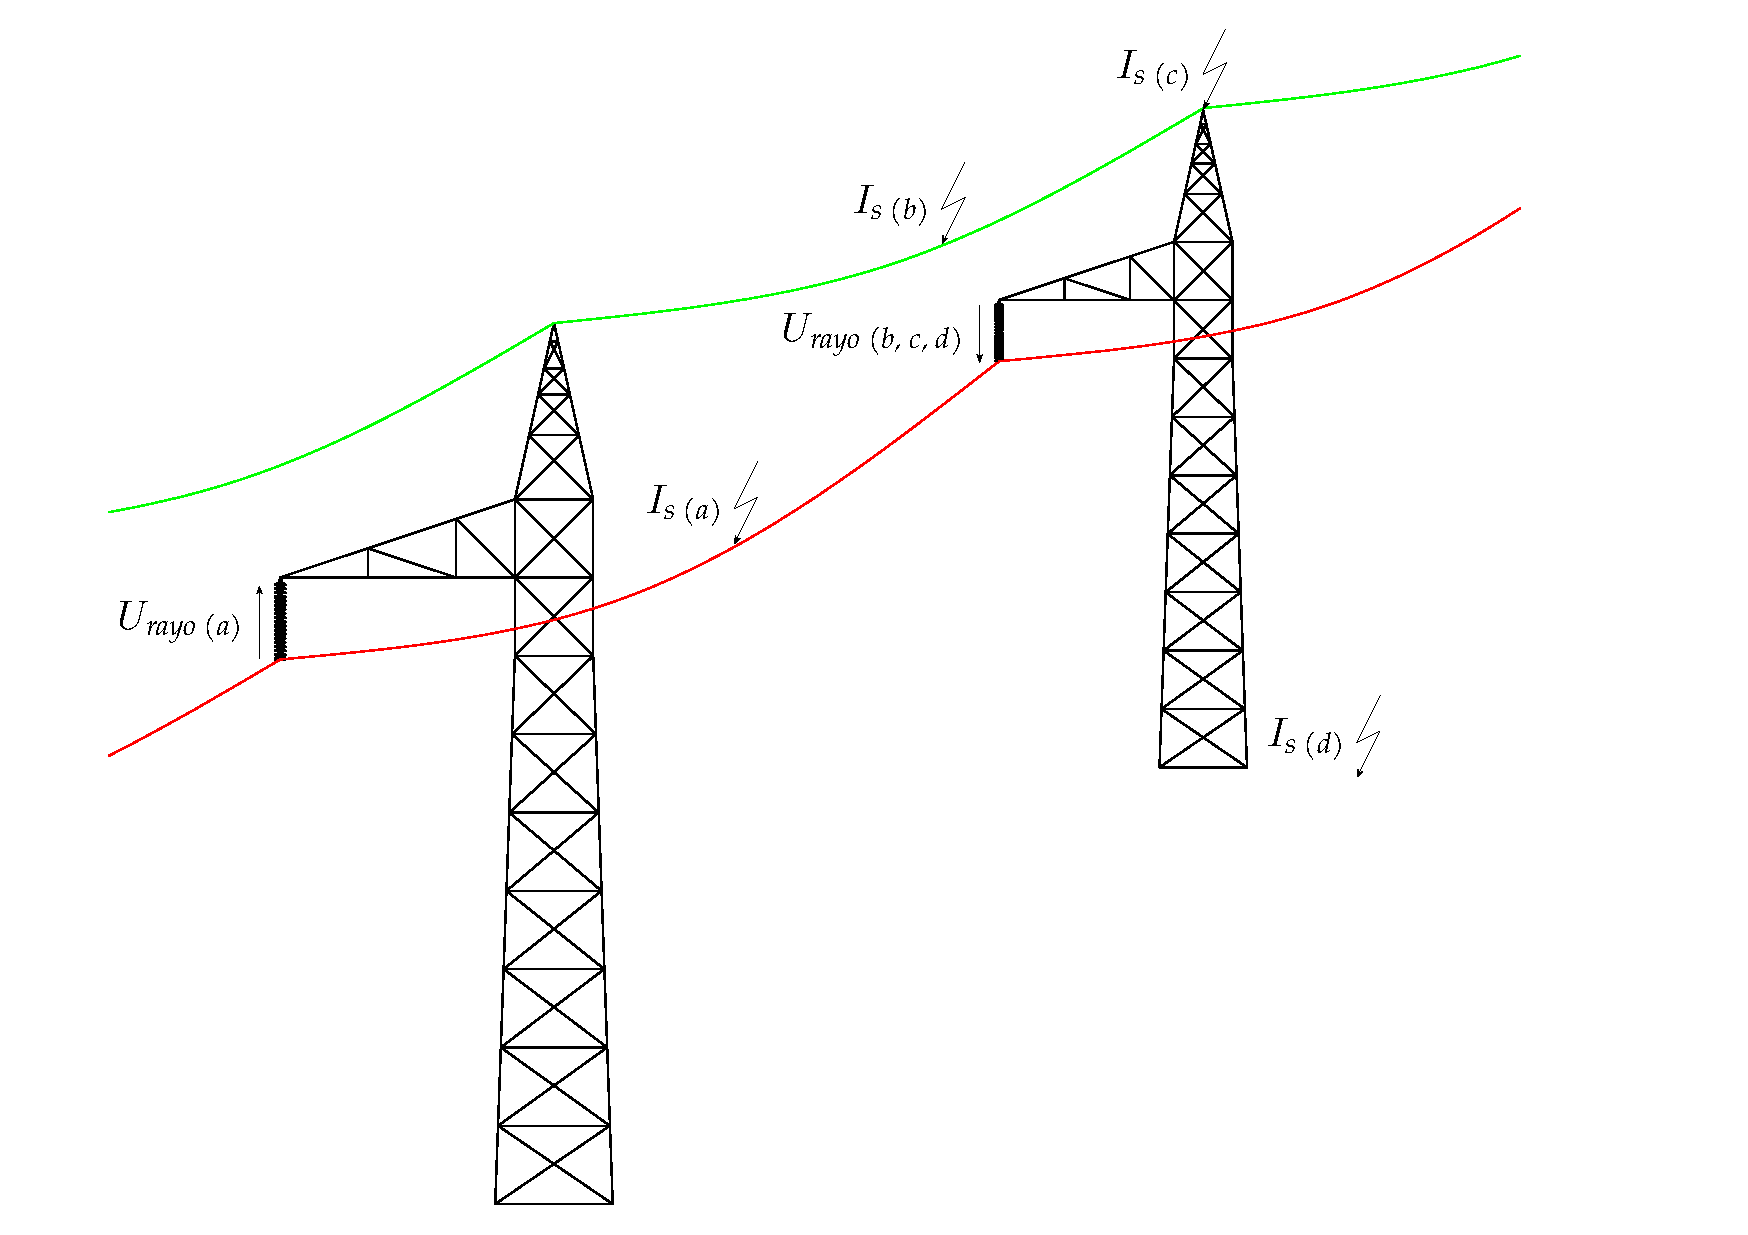
\includegraphics[scale=0.5]{capitulos/tema1/apoyoRayo/apoyoRayo.pdf}
                \caption{Caídas de rayo (sucesos independientes): a) Sobre el conductor activo. b) Sobre el cable de guarda.\\c) Sobre el apoyo. d) Sobre el terreno próximo.}
                \label{fig:caidaRayo}
            \end{figure}

            \textbf{\textit{El rayo impacta sobre un conductor fase.}} En este caso la corriente del rayo, $I_\textit{s}$, se divide en dos mitades aproximadamente iguales, $I_\textit{s}/2$, que viajaran a cada lado de la línea, ya que, tanto a un lado del punto de impacto como en el otro, la impedancia onda de la línea es similar. La mitad de la corriente que se propaga a cada lado de la línea provocará una tensión viajera, resultante de multiplicar la corriente $I_\textit{s}/2$ por la impedancia de onda, $Z$.\newline
            
            Por ejemplo, si impacta un rayo de $2\,\textit{kA}$, $1\,\textit{kA}$ viajará a cada lado de línea. Asumiendo que la impedancia de onda de la línea fuera de $400\,\Omega$, resultarían $400\,\textit{kV}$ de tensión viajara a cada lado. Si en lugar de impactar un rayo de $2\,\textit{kA}$ impactara uno rayo de amplitud diez veces mayor, $20\,\textit{kA}$, en vez de viajar una tensión de $400\,\textit{kV}$, viajarían una tensión de $4\,\textit{MV}$.\newline
            
            Evidentemente, dependiendo del nivel de sobretensión tipo rayo que viaje por la línea, podrá hacerlo sin provocar fallo de aislamiento o provocará la descarga disruptiva en la onda viajera, creando un impulso de tensión cortado en el frente en la cresta o después de la cresta (ver Fig. \ref{fig:graficaCebado}). El nivel de tensión de $4\,\textit{MV}$ es tan elevado que no podría ser soportado por la cadena de aisladores que sustenta a la línea en el apoyo, por lo que se provocará un cebado entre el conductor y el apoyo, generando un impulso de tensión cortado en el frente viajero por la línea.\newline
            
            \begin{figure}[H]
                \centering
                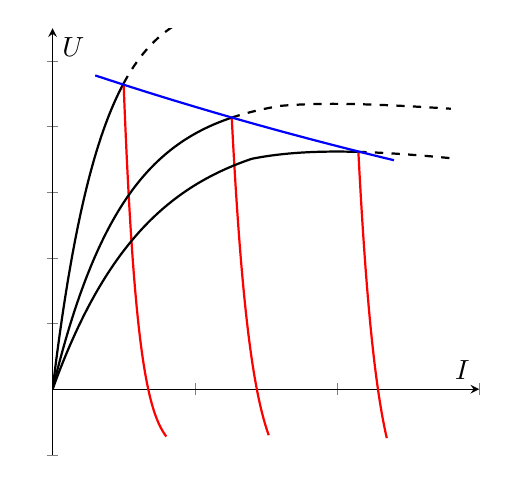
\begin{tikzpicture}
                    \begin{axis}[
                        axis lines = middle,
                        xlabel = $I$,
                        ylabel = $U$,
                        xmin=0, xmax=15,
                        ymin=-2, ymax=11,
                        xticklabels=none,
                        yticklabels=none,
                        domain=0:15,
                        samples=200,
                        width=7cm,
                        height=7cm,
                    ]
                    \addplot[black, thick, domain=0:2.5] {12 * (1 - exp(-0.6 * x))};
                    \addplot[black, thick, dashed, domain=2.5:4.5] {12 * (1 - exp(-0.6 * x))};
                    \addplot[red, thick, domain=2.5:4] {11.25 * (exp(-2*(x-2.5)))-2};
                    
                    \addplot[black, thick, domain=0:6.3] {9 * (1 - exp(-0.4 * x)) - 0.07 * (x - 8) * (x > 8)};
                    \addplot[black, thick, dashed, domain=6.3:14] {9 * (1 - exp(-0.4 * x)) - 0.07 * (x - 8) * (x > 8)};
                    \addplot[red, thick, domain=6.3:7.6] {11.25 * (exp(-1.5*(x-6.3)))-3};
                    
                    \addplot[black, thick, domain=0:10.75] {8 * (1 - exp(-0.3 * x)) - 0.12 * (x - 7) * (x > 7)};
                    \addplot[black, thick, dashed, domain=10.75:14] {8 * (1 - exp(-0.3 * x)) - 0.12 * (x - 7) * (x > 7)};
                    \addplot[red, thick, domain=10.75:11.75] {11.25 * (exp(-1.5*(x-10.75)))-4};
                    
                    \addplot[blue, thick, domain=1.5:12] {10 * exp(-0.03 * x)};
                    \end{axis}
                \end{tikzpicture}
                \caption{Impulsos de tensión tipo rayo cortados en el frente, en la cresta o después de la cresta, por el cebado de sus cadenas de aisladores.}
                \label{fig:graficaCebado}
            \end{figure}

            \textbf{\textit{El rayo impacta sobre el cable de guarda o el apoyo.}} El valor de la impedancia de onda del cable de guarda y apoyo es mucho bajo que el del conductor de fase de la línea y, por lo tanto, la sobretensión será menor. Si la tensión resultante fuera insuficiente para provocar la descarga disruptiva de la cadena de aisladores no se provocará sobretensión en los conductores de fase. Los conductores de fase solo sufrirán sobretensión si la amplitud del rayo fuera tan elevada como para provocar fallo en la cadena de aisladores o en la distancia libre de aire entre el apoyo (eleva su potencial) y uno de los conductores de fase.\newline
            
            Cuando el fallo es debido a la elevación de potencial de la estructura del apoyo (puesto a tierra) por el paso de la corriente del rayo se denomina \textit{cebado inverso}.\newline
            
            \textbf{\textit{El rayo impacta en el terreno próximo al apoyo.}} En estos casos la sobretensión que se inducen en la línea es del orden de algunos pocos de cientos de \textit{kV} (del orden de $100$ a $200\,\textit{kV}$)\footnote{Según Rusck, la tensión inducida $U(x)$ en un conductor de una línea situado a una altura $h\,[\textit{m}]$ cuando un rayo de intensidad $I\,[kA]$ descarga sobre el terreno próximo de resistividad $\rho\,(\Omega\cdot\textit{m})$ a una distancia $x\,[\textit{m}]$ del conductor viene dada por la expresión siguiente (ver tema 6): $$U(x) = \dfrac{Z_0\cdot I\cdot h_e}{x}\cdot \left[1+\dfrac{\dfrac{v}{v_0}}{\sqrt{2-\left(\dfrac{v}{v_0}\right)^2}}\right]$$ Donde $Z_0$ es la impedancia de onda del aire ($\approx 30\,\Omega$), $\dfrac{v}{v_0} = \dfrac{0.486}{1+\dfrac{27.3}{I}}$ y $h_e = h + \dfrac{4.7}{\sqrt{\dfrac{1000}{\rho}}}$}.\newline

            Esto significa que las líneas de media tensión, cuyo nivel de aislamiento no es superior de $125\,\textit{kV}$, fallarían cuando un rayo cayera en el terreno próximo a la línea. Este es el motivo por el cual las redes de media tensión no se apantallan habitualmente, pues lo estén o no lo estén las probabilidades de que su aislamiento falle en caso de rayos es muy alta.\newline
            
            Las sobretensiones del frente rápido que pueden aparecer en una subestación dependen del número de las líneas que se conectan a la subestación. Cuanto mayor sea el número de líneas que lleguen a la subestación mayor será la probabilidad que aparezca una sobretensión transmitida por una u otra línea. Si se trata de líneas de gran longitud, que además transcurren por zonas de gran densidad impactos de rayos, con estadísticas históricas de alto número de impactos por $\textit{km}^2$ y año, la probabilidad de sobretensiones en la subestación aumentará. También dependerá del mejor o peor apantallamiento de las líneas aéreas (ver tema 6).\newline
            
            El número de unidades de aisladores que componen las cadenas de aisladores afectará al valor máximo de la sobretensión que llega a la subestación. Si el número de aisladores está sobredimensionado (exceso del número aisladores), la cadena de aisladores soportará una mayor sobretensión y, en caso de una caída de tensión sobre un conductor de fase, se propagará a la subestación con un mayor nivel de sobretensión, al no descargar la cadena de aisladores. Si, por el contrario, el número de aisladores es demasiado pequeño, se producirá el contorneo de la cadena de aisladores para sobretensiones inferiores, de forma que no podrán propagarse sobretensiones superiores al nivel de tensión de contorneamiento de la cadena de aisladores\footnote{La norma UNE-EN 60071-2 estima que la tensión de probabilidad del $50\!$\% en descargar (rigidez dieléctrica) de las cadenas de aisladores de las líneas aéreas para rayos de polaridad negativa viene dada por la expresión. Se considera que la línea está situada a nivel del mar, en caso de otras altitudes debe corregirse esta tensión (ver Tema 7). $$U_{50\!\text{\%}}\,[\textit{k}\!\mathit{\hat{V}}] = 700\cdot d\,[\textit{m}]$$}.\newline

            Las sobretensiones que llegan a la subestación, si alcanzan valores excesivos para el material, deben ser limitadas por los pararrayos. La función de los pararrayos es reducir la sobretensión por debajo del nivel del aislamiento del material al que protege, tales como los transformadores de potencia y los cables de alta tensión, de tal manera que la tensión residual limitada por el pararrayos pueda ser soportada por el transformador o el cable al que protege.\newline

            Las cadenas de aisladores se eligen de nivel de aislamiento nominal para que las máximas sobretensiones tipo rayo que viajen queden recortadas por la cadena aisladores y, por lo tanto, el pararrayos de la subestación tendrá que drenar una energía limitada por la longitud de las cadenas de aisladores. Si el nivel de aislamiento nominal de las cadenas de aisladores se reduce, el pararrayos de la subestación drenará menos energía, aspecto positivo para el pararrayos, pero negativo para línea, ya que sufriría una tasa de fallos por año y \textit{km} demasiado elevada, afectando negativamente a la calidad de suministro. Por lo tanto, la elección del nivel de aislamiento es un compromiso entre limitar las sobretensiones que viajen por la línea y que no se produzcan excesivos fallos por año y \textit{km} en la línea\footnote{En determinados países con niveles ceraúnicos elevados (gran tasa de rayos por año y $\textit{km}^2$), en el lugar donde se produzcan numerosos cebados en las cadenas de aisladores de la línea y tener una tasa muy alta de fallos por año y $\textit{km}$ se utilizan pararrayos de línea, con el fin de limitar la sobretensión en las cadenas de aisladores y evitar que se produzca un fallo fase-tierra en la cadena de aisladores (los pararrayos limitan la sobretensión sin provocar un cortocircuito a tierra).}.\newline

        \subsection{Sobretensiones de frente muy rápido.}
            Las sobretensiones de frente muy rápido se producen en las subestaciones de alta tensión aisladas en gas (GIS) a alta presión (del orden de $6\,\textit{bar}$), por ejemplo en $\textit{SF}_6$ u otros gases alternativos más ecológicos para evitar el efecto invernadero. También en estas subestaciones se pueden producir el resto de sobretensiones (temporales y transitorias).\newline

            Estas sobretensiones se producen con motivo de maniobras de energización de las subestaciones aisladas en gas, por ejemplo, en la maniobra de cierre de los seccionadores inmersos en gas a alta presión. El escalón de tensión que se produce en la maniobra de cierre, desde el cero de tensión (fuera de servicio) hasta la tensión de la red, que en el caso más desfavorable puede alcanzar $U_\textit{s}\cdot \sqrt{2}/\sqrt{3}$ , provoca una onda de frente escarpado de tiempos de subida de nanosegundos. Este rápido frente de onda viaja entre el conductor y el conducto de la GIS.\newline

            Las GIS de $220\,\textit{kV}$ están blindadas en cada fase con conductos de un diámetro aproximado de unos $0.5\,\textit{m}$ que integran en su interior los conductores de fase, los seccionadores, los interruptores automáticos, los transformadores de tensión y de corriente para la medida y protección, etc. Las impedancias de onda de estos elementos pueden ser muy diferentes, lo que provoca que la onda de tensión viajera superponga reflexiones debido al cambio de impedancia de onda. Los codos de los conductos son cambios importantes de curvatura que, junto con los diferentes elementos de la GIS, son causa de reflexiones múltiples de las ondas viajeras, dando lugar a diferentes modos de propagación electromagnética. Esto hace que las sobretensiones que aparecen en estas instalaciones sean sobretensiones con ondas arbitrarias, con componentes frecuenciales muy elevadas, superpuestas, con tiempos de frente muy breves difícil de predecir.

        \subsection{Normalización de sobretensiones.}
            La norma UNE-EN 60071-2 clasifica y normaliza las sobretensiones según se muestra en la Tabla \ref{tab:sobretensionesNorma}. En esta tabla se resumen las tensiones y sobretensiones que aparecen en las redes eléctricas de alta tensión. En la primera columna se establecen las características a analizar de cada tipo de tensión y sobretensión, rango de variación, formas de ondas normalizadas y ensayos de tensión soportada normalizadas. La segunda columna de la tabla corresponde a la tensión permanente de la red que el material debe soportar de forma continuada en condiciones normales de servicio. Las normas particulares de cada material especifican el ensayo representativo en las condiciones de explotación de la red, carga y duración, para demostrar que el material ha sido diseñado y fabricado correctamente. La forma de onda de ensayo para esta tensión permanente es sinusoidal de $50$ ó $60\,\textit{Hz}$, dependiendo de la red a la que vaya a ser destinado. En las cuatro últimas columnas se resumen las sobretensiones temporales y las tres transitorias (de frente lento, frente rápido y de frente muy rápido).\newline

            {\noindent\centering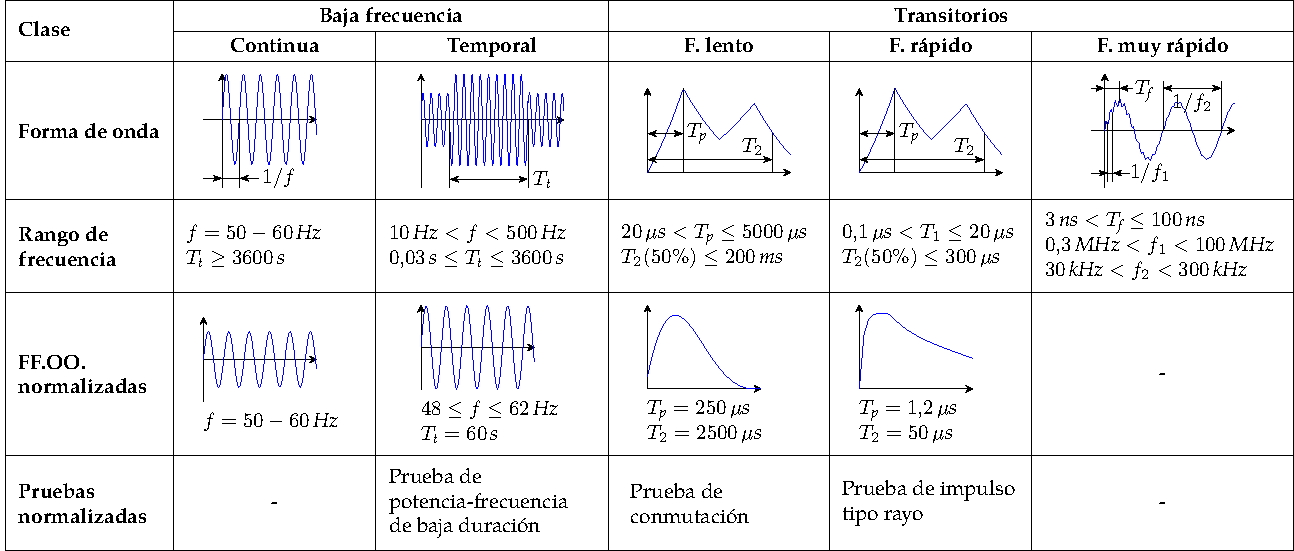
\includegraphics[scale=0.7]{capitulos/tema1/sobretensionesNorma/sobretensionesNorma.pdf}}
            \begin{table}[H]
                \caption{Clasificación y normalización de sobretensiones.}
                \label{tab:sobretensionesNorma}
            \end{table}

            \vspace{-0.5cm}
            En la primera fila se muestra la forma de las ondas de la tensión o sobretensión que pueden presentarse en la red. En la segunda fila se muestran los rangos de variación de los parámetros temporales o frecuenciales de estas formas de onda. En la tercera fila se muestran las formas de la onda normalizadas y sus parámetros asociados, que representan cada uno de los tipos de tensiones y sobretensiones y la última fila se especifica el nombre normalizado del ensayo de tensión soportada que demuestra que el aislamiento es capaz de soportar un cierto nivel de tensión para el tipo de tensión o sobretensión en consideración asociado al aislamiento correspondiente.\newline

            \begin{itemize}
                \item \textbf{\textit{Sobretensiones temporales.}} Corresponden a
                ondas sinusoidales con rangos de las frecuencias que pueden variar de $10\,\textit{Hz}$ hasta $500\,\textit{Hz}$. Las duraciones de estas sobretensiones pueden variar desde $30\,\textit{s}$ hasta una hora. Las forma de onda normalizada para todo este tipo de sobretensiones es una onda sinusoidal, de frecuencia comprendida entre $48$ y $62\,\textit{Hz}$, con una duración del ensayo normalizado de un minuto. La denominación normalizada del ensayo es \textit{ensayo de frecuencia industrial de corta duración}, y se realiza bajo lluvia normalizada para el material de exterior y en seco para el de interior\footnote{Pueden admitirse ensayos a frecuencias fuera del rango de frecuencia de los $48\,\textit{Hz}$ a $62\,\textit{Hz}$ cuando se hacen ensayos en campo, como es el caso de recepción de sistemas de cables de alta tensión, para los que se utilizan generadores resonantes de alta tensión que trabajan a frecuencias comprendidas entre $30\,\textit{Hz}$ y $300\,\textit{Hz}$.}.
                
                \item \textbf{\textit{Sobretensiones de frente lento.}} En las sobretensiones de frente lento se incluyen cualquier onda unidireccional cuyo tiempo hasta la cresta $T_\textit{p}$ sea mayor a $20\,\mu\textit{s}$, pero no superiores a $5\,\textit{ms}$ y con un tiempo hasta valor mitad de la cresta, $T_2$, inferior de $20\,\textit{ms}$. Como ya se ha indicado, estas sobretensiones tienen una duración de unos pocos de milisegundos, y la onda normalizada correspondiente al \textit{ensayo de tensión soportada a impulsos maniobra} es una onda de $T_\textit{p} = 250\,\mu\textit{s}$ y $T_2=2500\,\mu\textit{s}$ (onda 250/2500).
                
                \item \textbf{\textit{Sobretensiones de frente rápido.}} En el grupo de sobretensiones de frente rápido se encuentran todos los impulsos unidireccionales que tengan un tiempo de frente $T_1$ superior a $0.1\,\mu\textit{s}$, pero inferior a $20\,\mu\textit{s}$, y un tiempo hasta el valor mitad de la cresta $T_2$ inferior a $300\,\mu\textit{s}$. Los impulsos tipo rayo se normalizan por una onda $1.2/50$, es decir, una onda de tiempo de frente $T_1=1.2\,\mu\textit{s}$ y tiempo hasta el valor mitad $T_2=50\,\mu\textit{s}$. El ensayo normalizado se denomina de \textit{ensayo de tensión soportada a impulsos tipo rayo}.
                
                \item \textbf{\textit{Sobretensiones de frente muy rápido.}} Las solicitaciones de frente muy rápido son ondas con tiempos de frente $T_1$ del orden de nanosegundos (entre $100$ y $3\,\textit{ns}$), y las frecuencias de oscilación representativas son frecuencias del orden de \textit{MHz}. No existe un ensayo normalizado representativo para estas sobretensiones. Los ensayos de tensión soportada de impulsos tipo rayo y de impulsos maniobra son suficientes para demostrar que el material también podrá soportar las sobretensiones de frente muy rápido.
            \end{itemize}

            Solo las sobretensiones temporales deben ser soportadas por los materiales instalados en una red o subestación, pero las sobretensiones transitorias que aparecen en la red pueden ser superiores a las que sean capaces de soportar.\newline
            
            La norma UNE-EN 60071-2 exige que los materiales soporten hasta un cierto nivel las tensiones transitorias, pero si en la instalación se prevé que éstas sean superiores a las que puede soportar el material y como consecuencia de ello el material puede quedar dañado, entonces se precisará utilizar pararrayos. Tal es el caso de ciertos equipos o materiales (cables de alta tensión, transformadores de potencia, etc.), que deberán ser protegidos por pararrayos según se explica en tema 6. Sin embargo, otros materiales con aislamiento autorregenerable, tales como las cadenas de aisladores de vidrio, aisladores soporte de porcelana, no precisan, en general, de protección alguna de pararrayos.

    \section{Niveles de aislamiento nominales.}
        Una vez descritos los tipos de sobretensiones que se producen en las redes de alta tensión y presentados los ensayos normalizados asociados a estas sobretensiones se repasan los requisitos establecidos por el reglamento de instalaciones eléctricas de alta tensión. El reglamento, en su ITC 12, establece los niveles de aislamiento nominales para los diferentes grupos de materiales (A, B y C).\newline

        Los valores de las tensiones que deben soportar los aislamientos son valores normalizados. No se admiten elegir valores intermedios a los indicados en las Tablas \ref{tab:tensionesSoportadasA}, \ref{tab:tensionesSoportadasB} y \ref{tab:tensionesSoportadasC}. El nivel de aislamiento nominal debe ser elegido en función del correspondiente estudio de coordinación de aislamiento a realizar para cada instalación de alta tensión (ver tema 7). En caso de no haber realizado estudio de coordinación de aislamiento será necesario elegir el valor máximo de la tabla, es decir, la última fila para cada una de las $U_\textit{m}$.  

        \subsection{Niveles de aislamiento nominales para los materiales del Grupo A.}
            Para el material del grupo A, los ensayos se especifican con el fin de comprobar que el aislamiento es capaz de soportar los niveles de tensión especificados, en particular los devanados y los arrollamientos de las máquinas eléctricas (transformadores de distribución, generadores), que deben ser capaces de soportar las sobretensiones de origen atmosférico y sobretensiones de maniobras, especialmente debidas a recebados entre contactos de los aparatos de maniobra.\newline
            
            El reglamento establece para el material del grupo A dos listas: La lista 1 es de menor exigencia de aislamiento y la lista 2 de mayor exigencia. La elección del nivel de aislamiento de una u otra lista debe efectuarse en función del grado de exposición a sobretensiones tipo rayo y de maniobra, de la forma de puesta a tierra del neutro de la red y de los dispositivos de protección contra sobretensiones que existan. Todo ello con el fin de que exista una coordinación entre el nivel de aislamiento nominal capaz de soportar el material y las tensiones limitadas por los pararrayos (ver tema 7).\newline
            
            En la tabla \ref{tab:tensionesSoportadasA} se muestran los niveles de aislamiento nominal a frecuencia industrial y de impulsos tipo rayo para el material del grupo A. Para cada nivel de $U_\textit{m}$ hay un solo valor de tensión de ensayo a frecuencia industrial, pero al menos dos niveles de impulsos tipo rayo a elegir, uno de menor exigencia y otro de mayor exigencia, excepto para el caso de los materiales de $24\,\textit{kV}$, para el que existen dos valores de tensión de la lista 2 (mayor exigencia): $125\,\textit{kV}$ y $145\,\textit{kV}$.\newline
            
            Además, para el material del grupo A no se establecen diferencias entre las distancias libres en aire entre fase y tierra y distancias mínimas libres entre fases. Se especifican para la lista 1 distancias mínimas en aire menores cuando la instalación es de interior que cuando es de exterior, aunque para el material de $U_\textit{m}=24\text{ y }36\,\textit{kV}$ estas distancias son iguales, independientemente que se trate de instalaciones de interior o de exterior.\newline
            
            Cabe destacar que en los materiales del grupo A se establecen dos tensiones nominales de aislamiento: la \textit{tensión soportada a frecuencia industrial} y la \textit{tensión soportada a los impulsos tipo rayo}. No se establece ningún valor de tensión soportada a impulsos tipo maniobra. Esto no significa que este material no esté sometido a sobretensiones de tipo maniobra, sino que si el material se ensaya y soporta las tensiones nominales de frecuencia industrial y de impulsos tipo rayo también soportará sobretensiones de maniobra de un cierto nivel considerado en la norma de coordinación de aislamiento, sin necesidad de realizar ningún ensayo específico de maniobra.\newline 

            \begin{table}[H]
                \centering
                \renewcommand{\arraystretch}{1.1}
                \scalebox{0.9}{%
                \begin{tabular}{|c|c|c|c|c|c|c|c|}
                    \hline
                    \multirow{3}{*}{$U_\textit{m}\,[\textit{kV}_\textit{ef}]$} & \multirow{3}{*}{$U_\textit{f.i.}\,[\textit{kV}_\textit{ef}]$} & \multicolumn{2}{c|}{$U_\textit{rayo}(1.2/50)\,[\textit{kV}_\textit{p}]$} & \multicolumn{4}{c|}{\parbox{7cm}{\vspace{2mm}\centering Distancia mínima de aislamiento en aire fase-tierra y fase-fase [\textit{mm}]\vspace{2mm}}}\\
                    \cline{3-8}
                     &  & \multirow{2}{*}{Lista 1} & \multirow{2}{*}{Lista 2} & \multicolumn{2}{c|}{Lista 1} & \multicolumn{2}{c|}{Lista 2}\\
                    \cline{5-8}
                     & & & & I. interior & I. exterior & I. interior & I. exterior\\
                    \hline
                    \multirow{2}{*}{$3.6$} & \multirow{2}{*}{$10$} & 20 & - & 60 & 120 & - & - \\
                                           &                       & - & 40 & -  &   - & 60 & 120 \\
                    \hline
                    \multirow{2}{*}{$7.2$} & \multirow{2}{*}{$20$} & 40 & - & 60 & 120 & - & - \\
                                           &                       & - & 60 & -  &   - & 90 & 120 \\
                    \hline
                    \multirow{2}{*}{$12$}  & \multirow{2}{*}{$28$} & 60 & - & 90 & 150 & - & - \\
                                           &                       & - & 75 & -  &   - & 120 & 150 \\
                    \hline
                    \multirow{2}{*}{$17.5$}& \multirow{2}{*}{$38$} & 75 & - & 120 & 160 & - & - \\
                                           &                       & - & 95 & -  &   - & 160 & 160 \\
                    \hline
                    \multirow{3}{*}{$24$}  & \multirow{3}{*}{$50$} & 95 & - & 160 & 160 & - & - \\
                                           &                       & - & 125 & -  &   - & 220 & 220 \\
                                           &                       & - & 145 & -  &   - & 270 & 270 \\
                    \hline
                    \multirow{2}{*}{$36$}  & \multirow{2}{*}{$70$} & 145 & - & 270 & 270 & - & - \\
                                           &                       & - & 170 & -  &   - & 320 & 320 \\
                    \hline
                \end{tabular}
                }
                \caption{Tensiones soportadas nominales a frecuencia industrial y a impulsos tipo rayo. Distancia mínima de asilamiento fase a tierra y entre fases para los materiales del grupo A.}
                \label{tab:tensionesSoportadasA}
            \end{table}

            En la tabla puede observarse que el valor de la tensión soportada a impulsos tipo rayo de la lista 2 para una determinada $U_\textit{m}$ corresponde con el mismo valor de la lista 1 para el material del siguiente nivel de tensión. Así, por ejemplo, la tensión soportada nominal de la lista 2 del material de $U_\textit{m}=17.5\,\textit{kV}$, es de $95\,\textit{kV}$, valor que coincide con la tensión nominal soportada de la lista 1 para el material de $U_\textit{m}=24\,\textit{kV}$.
        
        \subsection{Niveles de aislamiento nominales para los materiales del Grupo B.}
            En la Tabla \ref{tab:tensionesSoportadasB} se asocia, para cada nivel de $U_\textit{m}$ del grupo B, las tensiones soportadas nominales de frecuencia industrial y de impulsos tipo rayo. Este grupo corresponde a materiales por encima de $36\,\textit{kV}$ y hasta $245\,\textit{kV}$ de tensión más elevada de la red. La elección de las distancias mínimas en aire se establece en función de las sobretensiones tipo rayo nominales. Puede observarse que, para cada nivel de tensión más elevada de la red a partir de $123\,\textit{kV}$, inclusive, existen varias alternativas de niveles de aislamiento nominales. También puede observarse que las dos primeras filas de valores de tensiones soportadas nominales correspondientes al material de $U_\textit{m}=145\,\textit{kV}$ son coincidentes con las dos filas de valores de tensiones soportadas nominales del material $U_\textit{m}=123\,\textit{kV}$. Análogamente las dos primeras filas de tensiones soportadas nominales del material de $U_\textit{m}=170\,\textit{kV}$ son las mismas que las dos últimas del material de $U_\textit{m}=145\,\textit{kV}$. También, la primera fila de valores de tensiones soportadas nominales correspondiente al material de $U_\textit{m}=245\,\textit{kV}$ es coincidente con la última de valores de tensiones soportadas nominales del material de $U_\textit{m}=170\,\textit{kV}$V. Todo ello demuestra que puede existir niveles de aislamientos iguales para materiales de distinto valor de $U_\textit{m}$.\newline

            \begin{table}[H]
                \centering
                \renewcommand{\arraystretch}{1.1}
                \scalebox{0.9}{%
                \begin{tabular}{|c|c|c|c|}
                    \hline
                    $U_\textit{m}\,[\textit{kV}_\textit{ef}]$ & $U_\textit{f.i.}\,[\textit{kV}_\textit{ef}]$ & $U_\textit{rayo}(1.2/50)\,[\textit{kV}_\textit{p}]$ & \parbox{5cm}{\vspace{2mm}\centering Distancia mínima de aislamiento en aire fase-tierra y fase-fase [\textit{mm}]\vspace{2mm}}\\
                    \hline
                    52 & 95 & 250 & 480\\
                    \hline
                    72.5 & 140 & 325 & 630\\
                    \hline
                    \multirow{2}{*}{$123$} & 185 & 450 & 900\\
                    & 230 & 550 & 1100\\
                    \hline
                    \multirow{3}{*}{$170$} & 230 & 550 & 1100\\
                    & 275 & 650 & 1300\\
                    & 325 & 750 & 1500\\
                    \hline
                    \multirow{4}{*}{$245$} & 325 & 750 & 1500\\
                    & 360 & 850 & 1700\\
                    & 395 & 950 & 1900\\
                    & 460 & 1050 & 2100\\
                    \hline
                \end{tabular}
                }
                \caption{Tensiones soportadas nominales a frecuencia industrial y a impulsos tipo rayo. Distancia mínima de asilamiento fase a tierra y entre fases para los materiales del grupo B.}
                \label{tab:tensionesSoportadasB}
            \end{table}

            Al igual que para los materiales el grupo A, el reglamento indica para los del grupo B que no se pueden elegir niveles intermedios a los valores normalizados. Se aconseja que, en caso de redes con el neutro conectado a una bobina de extinción o en las instalaciones cuyo coeficiente de defecto a tierra sea superior a $1.4$, se elija el nivel de aislamiento más elevado previsto para ese material. También, al igual que para los materiales del grupo A, en los del grupo B se establece la misma distancia libre en aire para las distancias mínimas de separación fase-tierra que para las distancias mínimas entre fases. Las distancias libres se aplican cuando no es posible realizar los ensayos de tensión soportada frecuencia industrial, ni de impulsos tipo rayo.
        
        \subsection{Niveles de aislamiento nominales para los materiales del Grupo C.}
            Los ensayos de tensión soportada a impulsos tipo rayo e impulsos de maniobra son requeridos para los materiales del grupo C (ver tabla \ref{tab:tensionesSoportadasC}). El reglamento establece seis combinaciones posibles de tensiones soportadas, siendo la tensión soportada a impulsos tipo rayo diferente para cada una de ellas, mientras que los valores de la tensión soportada a los impulsos tipo maniobra son comunes para dos valores consecutivos de tensiones soportadas a impulsos tipo rayo.\newline
            
            A diferencia de los grupos A y B, para el material del grupo C se establecen valores diferentes de tensiones soportadas nominales para distancias de aislamiento fase-tierra y las distancias en aire entre fases, siendo superiores los valores de las tensiones soportadas a impulsos tipo maniobra entre fases que entre fase y tierra. También, a diferencia de los materiales de los grupos A y B, para los del grupo C se requieren distancias mínimas de aislamiento en aire entre fases diferentes a las de entre fase y tierra.\newline
            
            Solo para el material del grupo C el reglamento establece distancias mínimas en aire diferentes en función de la forma geométrica de los conductores que separan el espacio libre en aire. La forma geométrica de los electrodos en el caso de fase tierra pueden ser punta/estructura o conductor/estructura. Si se trata de punta/estructura significa que el campo eléctrico es más intenso (menos homogéneo) que con conductor/estructura, y por lo tanto es necesario mayor distancia de separación. Cuando el campo eléctrico es más homogéneo, con menor distancia es posible soportar el mismo nivel de tensión. Análogamente sucede para las distancias mínimas de aislamiento en aire entre fases. Por ejemplo, la configuración punta/conductor requiere mayores distancias mínimas de separación que conductor/conductor, ya que la configuración punta/conductor es menos homogénea que conductor/conductor.\newline

            \begin{table}[H]
                \centering
                \renewcommand{\arraystretch}{1.1}
                \scalebox{0.9}{%
                \begin{tabular}{|c|c|c|c|c|c|c|c|}
                    \hline
                    \multirow{3}{*}{\makecell{$U_\textit{m}$\\$[\textit{kV}_\textit{ef}]$}} & \multirow{3}{*}{\makecell{$U_\textit{rayo}(1.2/50)$\\$[\textit{kV}_\textit{p}]$}} & \multirow{3}{*}{\makecell{$U_\textit{man}(250/2500)$\\$[\textit{kV}_\textit{p}]$}} & \multicolumn{2}{c|}{\parbox{3.5cm}{\vspace{2mm}\centering Distancia mínima de aislamiento en aire fase-tierra [\textit{mm}]\vspace{2mm}}} & \multirow{3}{*}{\makecell{$U_\textit{man}(250/2500)$\\$[\textit{kV}_\textit{p}]$}} & \multicolumn{2}{c|}{\parbox{3cm}{\vspace{2mm}\centering Distancia mínima de aislamiento en aire fase-fase [\textit{mm}]\vspace{2mm}}}\\
                    \cline{4-5}\cline{7-8}
                    \makecell{\vspace{2mm}\makecell{\text{ }\\\text{ }}\vspace{2mm}} & & & \makecell{Cond.-\\est. [\textit{mm}]} & \makecell{Punta-\\est. [\textit{mm}]} & & \makecell{Cond.-cond.\\(||) [\textit{mm}]} & \makecell{Punta-\\cond [\textit{mm}]}\\
                    \hline

                    \multirow{6}{*}{420} & 1050 & \multirow{2}{*}{850} & 1900 & \multirow{2}{*}{2400} & \multirow{2}{*}{1360} & \multirow{2}{*}{2900} & \multirow{2}{*}{3400}\\
                    & 1175 & & 2200 & & & & \\
                    \cline{2-8}
                    & 1175 & \multirow{2}{*}{950} & 2200 & \multirow{2}{*}{2900} & \multirow{2}{*}{1425} & \multirow{2}{*}{3100} & \multirow{2}{*}{3600}\\
                    & 1300 & & 2400 & & & & \\
                    \cline{2-8}
                    & 1300 & \multirow{2}{*}{1050} & \multirow{2}{*}{2600} & \multirow{2}{*}{3400} & \multirow{2}{*}{1575} & \multirow{2}{*}{3600} & \multirow{2}{*}{4200}\\
                    & 1425 & & & & & & \\
                    \hline

                \end{tabular}
                }
                \caption{Tensiones soportadas nominales a impulsos tipo rayo y a impulsos tipo maniobra. Distancia mínima de asilamiento fase a tierra y entre fases para los materiales del grupo C.}
                \label{tab:tensionesSoportadasC}
            \end{table}

            El reglamento permite para los materiales del grupo C emplear combinaciones distintas de tensiones soportadas a las establecidas en la tabla \ref{tab:tensionesSoportadasC} cuando, debido a las características de la red o a los métodos elegidos para controlar las sobretensiones de maniobra o de rayo, quede justificado, siempre que se utilicen valores nominales de los que figuran en la tabla. El reglamento también permite que, para los materiales del grupo C, puedan coexistir varios niveles de aislamiento nominal en diferentes materiales pertenecientes a una misma instalación.

    \section{Ensayos de tensiones soportadas nominales.}
        Los ensayos de tensiones soportadas nominales aplicables a los distintos aparatos e instalaciones de alta tensión están destinados a la comprobación del nivel de aislamiento nominal de frecuencia industrial, de impulsos tipo rayo y de impulsos de tipo maniobra que sean de aplicación según el grupo al que pertenezca el material (A, B o C). Aunque en las redes pueden aparecer cualquier tipo de sobretensiones (temporales, de tipo rayo y de tipo maniobra), tan solo se establecen dos ensayos de tensión soportada nominales para los materiales de cada grupo. Si se realizan estos dos ensayos con resultado favorable, el material también sería capaz de soportar hasta un cierto nivel sobretensiones del tipo de sobretensión no ensayado. Es decir, para los materiales de los grupos A y B las sobretensiones debidas a maniobras no son ensayadas, pero serán soportadas hasta un cierto nivel, si el material ha superado los ensayos de tensión soportada nominal de frecuencia industrial y de impulsos tipo rayo. Análogamente, para el material del grupo C se sabe que soportarán las sobretensiones temporales de un cierto nivel que aparezcan en la red, si los ensayos de tensión soportada nominal a impulsos tipo rayo y a impulsos tipo maniobra han sido superados.\newline
        
        Para la realización de los ensayos de verificación del nivel de aislamiento nominal se debe seguir las recomendaciones establecidas en la norma UNE EN 60060-1 sobre técnicas de ensayos de alta tensión. Esta norma es una norma horizontal que establece los criterios y requisitos generales de los ensayos, tales como las formas de onda, tolerancias y métodos de ensayo. También debe seguirse la norma UNE EN 60071-2 sobre coordinación de aislamiento. Además, para cada tipo de material, aparato o instalación (aislador, cable, transformador de potencia, transformador de medida, fusible, etc.) debe aplicarse la norma UNE EN correspondiente\footnote{Ver listado de normas establecida en la ITC 02 del RAT.}. En estas normas se fijan aspectos específicos de las condiciones de los ensayos aplicables a cada material, tales como modo de instalación, condiciones de funcionamiento durante los ensayos, etc.\newline
        
        La normativa internacional considera como nivel de tensión soportada, $U_\textit{w}$, para los aislamientos de aire ambiente\footnote{El aire ambiente es un aislamiento autorregenerable que, tras una descarga disruptiva, recupera sus propiedades dieléctricas, al renovarse por aire ambiente circundante. Para aislamientos no autorregenerables, como dieléctricos sólidos y líquidos (resinas, materiales poliméricos, siliconas, aceite, papel-aceite, etc.) la tensión soportada corresponde al valor de truncamiento de la función de densidad de probabilidad: $$U_\textit{t} = (1-3\sigma)\cdot  U_{50\!\text{\%}}$$} el nivel de tensión cuya probabilidad de producir un cebado es el 10\!\%, $U_{10\!\text{\%}}$, lo que significa que la probabilidad de ser soportado es del 90\!\%. Asumiendo que la función densidad de probabilidad de la descarga disruptiva en aire sigue una evolución gaussiana se puede determinar la tensión de probabilidad de ser soportada del 10\!\% a través del valor tensión de probabilidad de ser soportada del 50\!\%, $U_{50\!\text{\%}}$, y su desviación típica $\sigma$\footnote{Según la norma UNE EN 60071-2, la desviación típica, $\sigma$, para las tensiones de frecuencia industrial e impulsos tipo rayo o maniobra de polaridad positiva puede considerase del orden del 3\!\%, mientras que para impulsos de polaridad negativa es del orden del 5\!\%. La presencia de aisladores incrementa la desviación típica de 5\!\% a 9\!\%.}:
        \begin{equation}
            U_{10\!\text{\%}} = (1-1.3\sigma)\cdot U_{50\!\text{\%}}
        \end{equation}

        \begin{figure}[H]
            \centering
            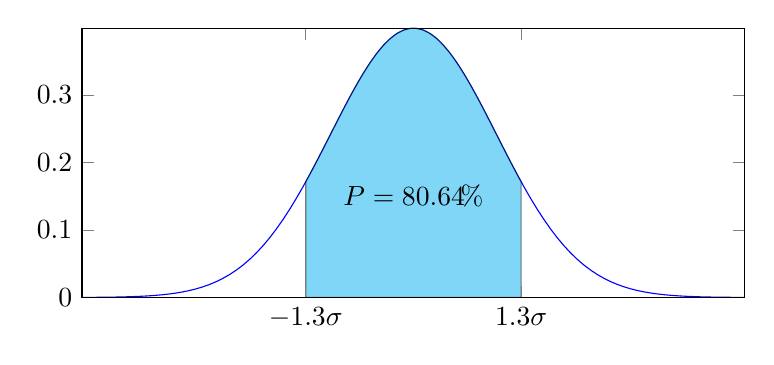
\begin{tikzpicture}
                \begin{axis}[
                    no markers,
                    domain=-4:4,
                    samples=100,
                    height=5cm, width=10cm,
                    xtick={-1.3,1.3},
                    xticklabels={$-1.3\sigma$, $1.3\sigma$},
                    enlargelimits=false,
                    clip=false,
                    axis on top,
                ]
                \addplot [blue] {exp(-x^2/2)/sqrt(2*pi)};
                \addplot [domain=-1.3:1.3,fill=cyan,opacity=0.5] {exp(-x^2/2)/sqrt(2*pi)} \closedcycle;
                \node at (axis cs:0,0.15)[]{$P=80.64\!\text{\%}$};
                \end{axis}
            \end{tikzpicture}
            \caption{Función densidad de probabilidad normalizada de una distribución normal ($U_{50\!\text{\%}}=1$).}
            \label{fig:distNormal}
        \end{figure}

        Uno de los métodos normalizados más habituales para determinar $U_{50\!\text{\%}}$, aplicable a las tensiones de impulsos tipo rayo y de tipo maniobra, es el \textit{método de subida y bajada}. Este método consiste en incrementar progresivamente el valor de la tensión de ensayo en una pequeña cantidad, $\Delta U$\footnote{la norma UNE-EN 60060-1 recomienda que $\Delta U$ esté comprendido entre el $1\!$\% y el $3\!$\% de $U_{50\!\text{\%}}$.}, desde un nivel de tensión algo inferior al estimado como $U_{50\!\text{\%}}$ hasta alcanzar la primera descarga. Tras la primera descarga, la tensión se reducirá $\Delta U$. Si al aplicar el nuevo nivel de tensión vuelve a producirse una descarga, se reducirá nuevamente la tensión otro escalón $\Delta U$, de lo contrario se incrementará $\Delta U$, de forma que detrás de una descarga la tensión se reduce $\Delta U$, y si no descarga (soporta) la tensión, se incrementa $\Delta U$. Tras un número suficientemente amplio de aplicaciones de tensión después de la primera descarga, por ejemplo, $m=50$, se determina la tensión $U_{50\!\text{\%}}$ como valor medio de las tensiones aplicadas:
        \begin{equation}
            U_{50\!\text{\%}} = \dfrac{\sum\limits_{i=1}^m U_i}{m}
        \end{equation}
        
    \section{Distancias en aire entre elementos en tensión y tierra.}
        \subsection{Relaciones entre las tensiones soportadas y las distancias en aire.}
            El anexo F de la norma IEC 60071-2 establece la formulación empírica que relaciona la tensión $U_{50\!\text{\%}}$ con la distancia de separación en aire para las ondas normalizadas de frecuencia industrial, impulsos tipo rayo y tipo maniobra. Estas fórmulas son aplicables a separaciones de aire punta-plano y distancias superiores a $1\,\textit{m}$:
            \begin{itemize}
                \item \textit{\textbf{Frecuencia industrial.}}
                \begin{equation}
                    U_{50\!\text{\%}}(\textit{f.i.})\,[\textit{kV}_\textit{ef}]= 750\cdot \ln(1+0.55\cdot d[\textit{m}]^{1.2})
                \end{equation}

                \item \textit{\textbf{Impulsos tipo rayo (1.2/50).}}
                \begin{equation}
                    U_{50\!\text{\%}}(\textit{rayo }1.2/50)\,[\textit{kV}_\textit{p}]= 530\cdot d[\textit{m}]
                \end{equation}

                \item \textit{\textbf{Impulsos tipo maniobra (250/2500).}}
                \begin{equation}
                    U_{50\!\text{\%}}(\textit{man. }50/2500)\,[\textit{kV}_\textit{p}]= 500\cdot d[\textit{m}]^{0.6}
                \end{equation}
            \end{itemize}

            Sin embargo, la separación obtenida no siempre corresponde a una configuración punta-plano, que es la más desfavorable. Cualquier otra configuración de electrodos para la misma distancia de separación soportará más tensión. Dependiendo de como sea la configuración de los electrodos que conforman la separación libre en aire, la tensión para impulsos tipo maniobra se incrementa en un factor $K$, denominado factor de separación. El resto de ensayos ven incrementada su tensión en relación a este mismo factor. En las tablas \ref{tab:coefsFT} y \ref{tab:coefsFF} se muestran factores de separación definidos en el anexo F de la norma, para las geometrías más usuales.

            \begin{table}[H]
                \centering
                \begin{tabular}{|l|c|}
                    \hline
                    \textbf{Tipo de separación}                           & \textbf{K}  \\ \hline
                    Conductor-cruceta                                     & 1,45        \\ \hline
                    Conductor-ventana                                     & 1,25        \\ \hline
                    Conductor-plano                                       & 1,15        \\ \hline
                    Conductor-estructura inferior en punta                & 1,47        \\ \hline
                    Conductor-estructura lateral                          & 1,45        \\ \hline
                    Longitudinal: Punta-estructura                        & 1,35        \\ \hline
                    \end{tabular}
                \caption{Coeficientes del factor de separación fase-tierra.}
                \label{tab:coefsFT}
            \end{table}

            \begin{table}[H]
                \centering
                \begin{tabular}{|l|c|}
                    \hline
                    \textbf{Tipo de separación}                                                   & \textbf{K}         \\ \hline
                    Anillo-Anillo o electrodos planos de gran tamaño                              & 1,70 -- 1,80       \\ \hline
                    Conductores cruzados                                                          & 1,53 -- 1,70       \\ \hline
                    Punta–punta o conductor-conductor (a lo largo del vano)                       & 1,62 -- 1,52       \\ \hline
                    Soporte de embarrados                                                         & 1,40 -- 1,50       \\ \hline
                    Geometrías Asimétricas                                                        & 1,36 -- 1,45       \\ \hline
                    \end{tabular}
                \caption{Coeficientes del factor de separación fase-fase.}
                \label{tab:coefsFF}
            \end{table}
            
            Luego las expresiones corregidas por el factor $K$ y la distribución normal resultan:
            \begin{itemize}
                \item \textit{\textbf{Frecuencia industrial.}}
                \begin{equation}
                    U_\textit{w}(\textit{f.i.})\,[\textit{kV}_\textit{ef}]=
                    (1-1.3\sigma)\cdot(1.35K-0.35K^2)\cdot[750\cdot \ln(1+0.55\cdot d[\textit{m}]^{1.2})]
                \end{equation}

                \item \textit{\textbf{Impulsos tipo rayo (1.2/50).}}
                \begin{equation}
                    U_\textit{w}(1.2/50)\,[\textit{kV}_\textit{p}]= 
                    (1-1.3\sigma)\cdot(0.74+0.26K)\cdot 530\cdot d[\textit{m}]
                \end{equation}

                \item \textit{\textbf{Impulsos tipo maniobra (250/2500).}}
                \begin{equation}
                    U_\textit{w}(50/2500)\,[\textit{kV}_\textit{p}]= 
                    (1-1.3\sigma)\cdot K\cdot 500\cdot d[\textit{m}]^{0.6}
                \end{equation}
            \end{itemize}

        \subsection{Elección de las distancias mínimas en aire reglamentarias.}
            Como ya ha sido indicado, una vez elegido el nivel de aislamiento para una instalación, el material elegido de un determinado grupo (A, B o C) debe soportar dos tensiones nominales de aislamiento. Por ejemplo, el material de $U_\textit{m}=145\,\textit{kV}$, perteneciente al grupo B, con el mayor nivel de aislamiento debe ser capaz de soportar una tensión nominal a frecuencia industrial de $275\,\textit{kV}$ y una tensión a impulsos tipo rayo de $650\,\textit{kV}$. Para el caso de los materiales del grupo C, el material deberán soportar una tensión nominal a impulsos tipo rayo, dos a impulsos tipo maniobra, una entre fase y tierra y la otra entre fase y fase. La pregunta que cabe plantearse es cuál de las tensiones nominales de aislamiento requeridas es la que impone la mayor distancia de separación en aire.\newline
            
            En la segunda, tercera y cuarta columnas de la tabla \ref{tab:distMinimas} se muestran las parejas de tensiones soportadas nominales de frecuencia industrial, impulsos tipo rayo e impulsos tipo maniobra asociadas a los materiales del grupo B y las correspondientes para un material del grupo C (última fila), que pueden ser comunes a diferentes $U_\textit{m}$ (ver primera columna). En la quinta columna se incluye la distancia mínima de aislamiento en aire reglamentaria para separaciones fase-tierra y separaciones entre fases para el material del grupo B y la distancia mínima de aislamiento en aire fase-tierra para la configuración punta/estructura del material del grupo C (última fila).\newline
            
            Teniendo en cuenta las expresiones presentadas que relacionan las tensiones soportadas, $U_\textit{w}$, con las distancias de separación, $d$, es posible determinar las distancias de separación asociadas a cada tensión nominal soportada reglamentaria: la distancia asociada a la tensión soportada nominal de frecuencia industrial (columna sexta), asociada a impulsos tipo rayo (columna séptima) y asociada a impulsos tipo maniobra (columna octava). Puede observarse que para el material del grupo B la tensión soportada nominal asociada a impulsos tipo rayo es la que impone la mayor distancia libre, mientras que para el caso del material del grupo C la que impone mayor distancia libre en aire es la tensión soportada nominal impulsos tipo maniobra.

            \begin{table}[H]
                \centering
                \renewcommand{\arraystretch}{1.1}
                \scalebox{0.9}{%
                \begin{tabular}{|c|c|c|c|c|c|c|c|}
                    \hline
                    $U_\textit{m}$ & $U_\textit{w (f.i.)}$ & $U_{\textit{w }(1.2/50)}$ & $U_{\textit{w }(250/2500)}$ & $d$ & $d(U_{\textit{w (f.i.)}})$ & $d(U_{\textit{w }(1.2/50)})$ & $d(U_{\textit{w }(250/2500)})$\\
                    $[\textit{kV}]$ & $[\textit{kV}]$ & $[\textit{kV}]$ & $[\textit{kV}]$ & $[\textit{m}]$& $[\textit{m}]$& $[\textit{m}]$& $[\textit{m}]$\\
                    \hline
                    $52$ & $95$ & $250$ & - & - & - & - & -\\
                    \hline
                    $72.5$ & $140$ & $325$ & - & - & - & - & -\\
                    \hline
                    $123$, $145$ & $185$ & $450$ & - & $0.9$ & $0.6$ & $0.9$ & -\\
                    \hline
                    $123$, $145$, $170$ & $230$ & $550$ & - & $1.1$ & $0.7$ & $1.1$ & -\\
                    \hline
                    $145$, $170$ & $275$ & $650$ & - & $1.3$ & $0.8$ & $1.3$ & -\\
                    \hline
                    $170$, $245$ & $325$ & $750$ & - & $1.5$ & $1.0$ & $1.5$ & -\\
                    \hline
                    \multirow{3}{*}{$245$} & $360$ & $850$ & - & $1.7$ & $1.1$ & $1.7$ & -\\
                    & $395$ & $950$ & - & $1.9$ & $1.2$ & $1.9$ & -\\
                    & $460$ & $1050$ & - & $2.1$ & $1.4$ & $2.1$ & -\\              
                    \hline      
                    $420$ & - & $1050$ & $850$ & $2.4$ & - & $2.1$ & $2.4$\\
                    \hline
                    \end{tabular}
                }
                \caption{Distancias mínimas de aislamiento en aire normalizadas y distancias libres en aire asociadas a las tensiones soportadas nominales de frecuencia industrial, de impulsos rayo y de impulsos tipo maniobra.}
                \label{tab:distMinimas}
            \end{table}

        \subsection{Requisitos reglamentarios sobre las distancias mínimas en aire.}
            Si no es posible efectuar los ensayos de tensión soportada se pueden guardar unas distancias mínimas en el aislamiento en aire que permiten garantizar los niveles de tensión soportada. Aunque las distancias mínimas dependen de las configuraciones de las partes activas y de las estructuras próximas, solo para los materiales del grupo C se recogen diferentes distancias en función del factor de separación $K$. Para el resto de los materiales correspondientes a los grupos A y B se utiliza la distancia más conservadora para cada nivel de aislamiento nominal.\newline

            No es necesario cumplir las distancias mínimas si existen ensayos de tensión soportada especificados en las normas particulares del material realizados con resultados favorables, puesto que ello entorpecería a su diseño, aumentaría su costo y dificultaría en progreso tecnológico.\newline

            Las distancias mínimas en el aire reflejadas en las tablas \ref{tab:tensionesSoportadasA}, \ref{tab:tensionesSoportadasB} y \ref{tab:tensionesSoportadasC} deben respetarse en los equipos e instalaciones donde no se hayan realizado ensayos que justifiquen que las tensiones soportadas nominales de su nivel de aislamiento se cumplen. Estas distancias especificadas son distancias en el aire sin en tener en consideración caminos de descarga por contorneo de un aislador. En el caso de los aisladores deberán efectuarse ensayos conforme a las normas específicas UNE EN 60168 y UNE EN 60507 de la línea de fuga. Esta última norma tiene en cuenta el fenómeno de contaminación por polución, que producen descargas a través de la superficie externa de los aislamientos que difieren de distancias en aire libres requeridas en las tablas anteriores. Las descargas por fenómenos de contaminación afectan a la longitud y forma de línea de fuga de los aisladores y deben ser satisfechas, además de las tensiones soportadas nominales o distancias mínimas en aire que establece el reglamento.\newline

            Asimismo, el reglamento establece que para separar eléctricamente circuitos se utilizan preferentemente seccionadores diseñados conforme a la norma correspondiente. No obstante, nos indica que también pueden lograrse la condición de seccionamiento sin necesidad de seccionador si las distancias entre los dos extremos seccionados de cada una de las fases se incrementa, al menos un $25$\!\% respecto a las distancias mínimas de aislamiento en el aire establecidas en las tablas \ref{tab:tensionesSoportadasA} y \ref{tab:tensionesSoportadasB}, para los grupos A y B, y para las distancias mínimas de aislamiento entre fases de la tabla \ref{tab:tensionesSoportadasC} para materiales del grupo C. Es decir, en el caso del grupo C, donde hay dos columnas de distancias de separación, una distancia fase-tierra y la otra distancia entre fases, se debe elegir la distancia entre fases, que requiere mayores valores, e incrementarla en un $25$\!\%, de tal manera que las sobretensiones en la red nunca podrán provocar una descarga entre los contactos separados esa distancia.\newline

            Las distancias que vienen en las tablas \ref{tab:tensionesSoportadasA}, \ref{tab:tensionesSoportadasB} y \ref{tab:tensionesSoportadasC} son valores mínimos determinados por consideraciones de tipo eléctrico, pero en algunos casos deben ser incrementadas para tener en cuenta otros conceptos como las tolerancias de construcción, los efectos de esfuerzos provocados por cortocircuitos, efectos del viento que pueden hacer moverse partes de conductores que no estén fijados de forma segura, etc. Estas distancias no se deben confundir con las distancias de seguridad del personal, tales como pasillos, que corresponden a otros criterios de diseño. Las distancias de proximidad y de trabajos con o sin tensión relacionadas con seguridad para las personas se rigen por Real Decreto 614.\newline

            Las distancias establecidas en las tablas \ref{tab:tensionesSoportadasA}, \ref{tab:tensionesSoportadasB} y \ref{tab:tensionesSoportadasC} son válidas para altitudes no superiores a $1000\,\textit{m}$. Para las instalaciones situadas por encima de esta altitud, las distancias mínimas en el aire, hasta los $3000\,\textit{m}$, deben aumentarse en un $1.4\!$\% por cada $100\,\textit{m}$, o fracción por encima de los $1000\,\textit{m}$\footnote{Este aumento de las distancias mínimas es debido a la reducción de la presión atmosférica. Conforme a lo establecido por la norma IEC 60071-2, la reducción de presión atmosférica, al aumentar la altitud, conduce a una reducción de la tensión soportada del aislamiento externo, que es determinada a través del factor de corrección atmosférica $K_\textit{a}$: $$K_\textit{a} = e^{-m\cdot h/8150}$$ Donde $h$ es la altitud sobre el nivel del mar $[\textit{m}]$ y $m$ es un factor que toma valores entre $0$ y $1$ en función del tipo de sobretensión (temporal, tipo rayo o tipo maniobra) y del valor de la sobretensión. La variación de la tensión soportada por cada metro de altitud incremental se determina derivando la expresión anterior: $$\dfrac{\partial K_\textit{a}}{\partial h} = -\dfrac{m}{8150}\cdot e^{-m\cdot h/8150}$$ Cuando $m=1$ se produce la mayor disminución de tensión soportada al incrementar la altitud, por lo que se tomará este valor como el más desfavorable. Esta variación, expresada en tanto por ciento: $$\left.\left(\dfrac{\partial K_\textit{a}}{\partial h}\cdot\dfrac{1}{K_\textit{a}}\right)\right|_{100\!\text{\%}} = -\dfrac{m}{8150}\cdot 100 = -0.0123\!\text{\%}$$ Tomando la referencia de incremento de altitud $100\,\textit{m}$ resulta: $$\left.\left(\dfrac{\partial K_\textit{a}}{\partial h}\cdot\dfrac{1}{K_\textit{a}}\right)\right|_{100\!\text{\%}} = -1.23\!\text{\%}\text{ por cada }100\,\textit{m}$$ Como ya ha sido indicado, las sobretensiones tipo maniobras son las que imponen las distancias de aislamiento mayores, siendo la relación entre las distancias libres en aire con las sobretensiones tipo maniobra: $U_{50\!\text{\%}} = 500\cdot d^{0.6}$. Por lo tanto, el incremento de distancia en aire para compensar la disminución de la tensión soportada será $$1.23^{1/0,6}=1.4\!\text{\%}\text{ por cada }100\,\textit{m}\text{ o fracción por encima de los }1000\,\textit{m}\text{ de altitud}$$\!}.